%%================================================
%% Filename: chap02.tex
%% Encoding: UTF-8
%% Author: Yuan Xiaoshuai - yxshuai@gmail.com
%% Created: 2019-11-10 10:32
%% Last modified: 2019-11-20 10:49
%%================================================
\chapter{模板使用示例 Some Examples}
\label{cha:examples}

\section{插图示例}
\label{sec:figure}

\subsection{插入单幅图形}

插图通常需要占据大块空白,所以在文字处理软件中用户经常需要调整插图的位置。
\LaTeX~有一个 \texttt{figure} 环境可以自动完成这样的任务,这种自动调整位置的环
境称作浮动环境(float),之后还会介绍表格浮动环境。

单张图片插入形式如图~\ref{fig:golfer}~所示。
\begin{figure}[htbp]
\centering
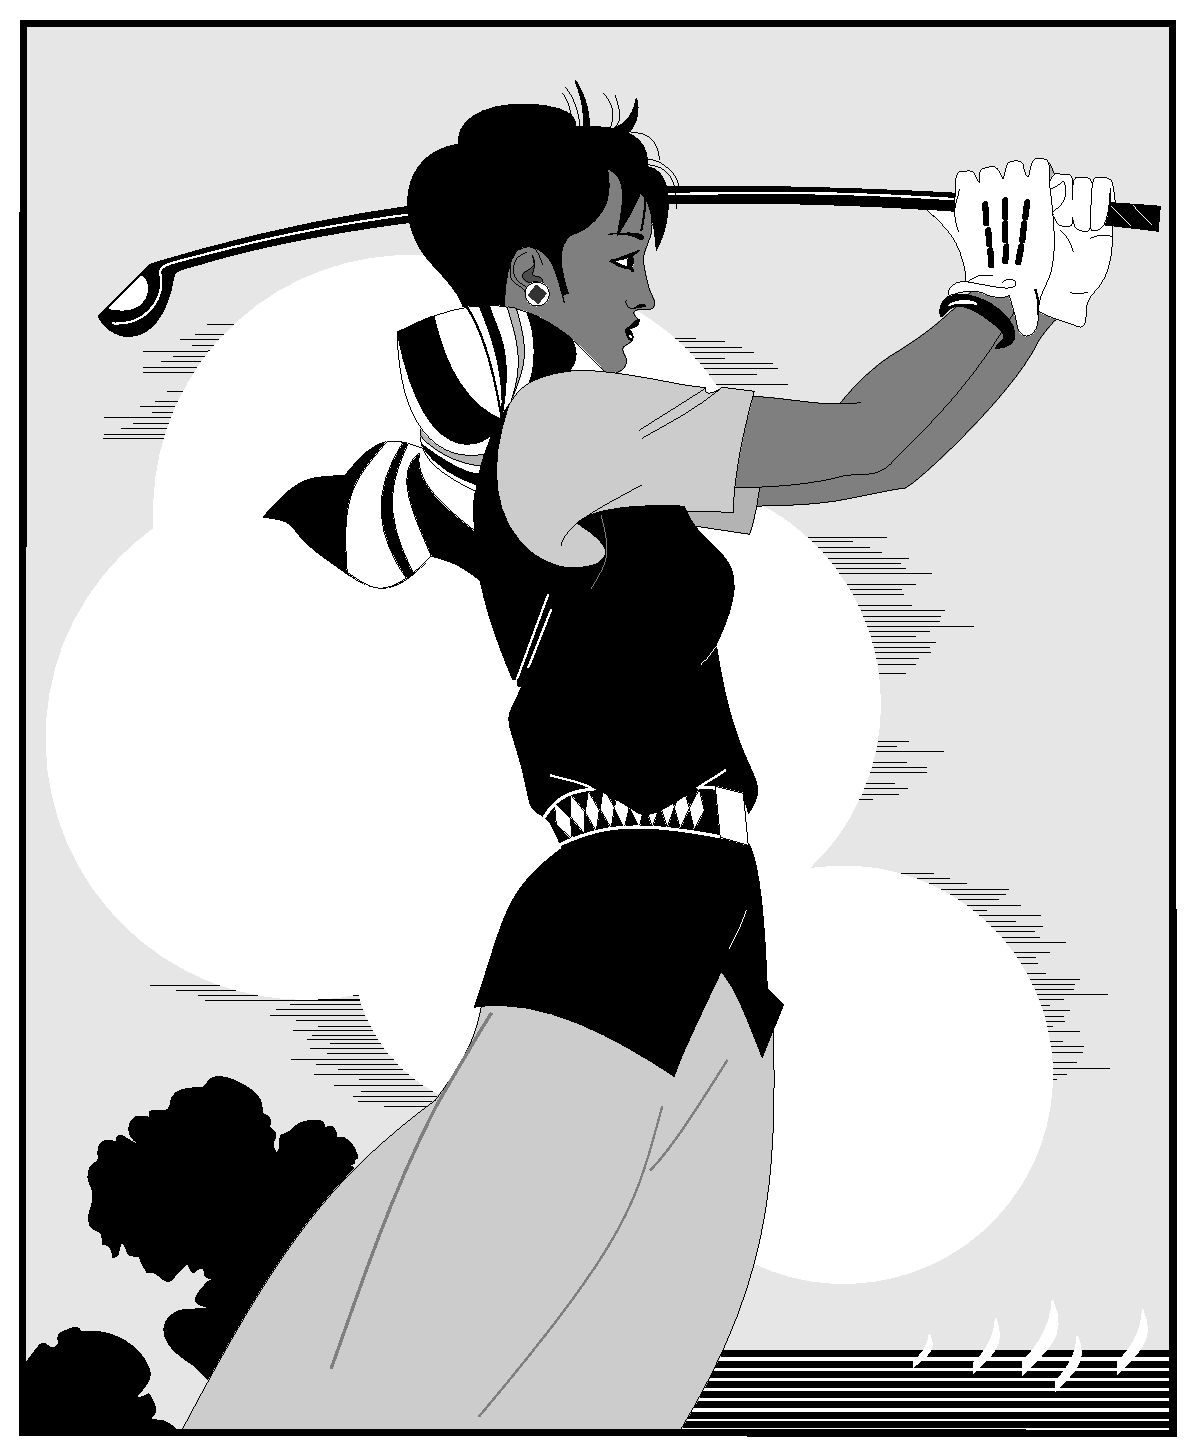
\includegraphics[width = 0.3\textwidth]{golfer}
\bicaption{打高尔夫球的人}
          {Golfer}
\label{fig:golfer}
\end{figure}

\subsection{插入多幅图形}

\subsubsection*{并排摆放,共享标题}

当我们需要两幅图片并排摆放,并共享标题时,可以在 \texttt{figure} 环境中使用两个
插图命令,如图~\ref{fig:fanqingfuming}~所示。

\begin{figure}[htbp]
\centering

\includegraphics[width=0.3\textwidth]{qingming}
\hspace{36pt}

\includegraphics[width=0.3\textwidth]{fanfu}
\bicaption{反清复明}{Fan Qing Fu Ming}
\label{fig:fanqingfuming}
\end{figure}

\subsubsection*{并排摆放,各有标题}

如果想要两幅并排的图片各有自己的标题,可以在 \texttt{figure} 环境中使用两个
 \texttt{minipage} 环境,每个环境里插入一个图,如图~\ref{fig:qingming}~和
~\ref{fig:fanfu}~所示。

\begin{figure}[htbp]
\centering
\begin{minipage}[t]{0.3\textwidth}
    \centering
    
\includegraphics[width=\textwidth]{qingming}
    \bicaption{清明}{Qing Ming}
    \label{fig:qingming}
\end{minipage}
\hspace{36pt}
\begin{minipage}[t]{0.3\textwidth}
    \centering
    
\includegraphics[width=\textwidth]{fanfu}
    \bicaption{反复}{Fan Fu}
    \label{fig:fanfu}
\end{minipage}
\end{figure}

\subsubsection*{并排摆放,共享标题,各有子标题}

如果想要两幅并排的图片共享一个标题,并各有自己的子标题,可以使用 \textbf{subcaption} 宏包提供的 \texttt{subcaptionbox} 命令,每个子图可以有各自的引用,如图~\ref{fig:subfig_a}~和~\ref{fig:subfig_b}~所示。

\begin{figure}[htbp]
\centering
\bisubcaptionbox{清明\label{fig:subfig_a}}{Qing Ming}[0.3\textwidth]{
    
\includegraphics[width=0.3\textwidth]{qingming}
}
\hspace{36pt}
\bisubcaptionbox{反复\label{fig:subfig_b}}{Fan Fu}[0.3\textwidth]{
    
\includegraphics[width=0.3\textwidth]{fanfu}
}
\bicaption{反清复明}{Fan Qing Fu Ming}
\end{figure}

\section{表格示例}
\label{sec:table}

\subsection{普通表格的绘制方法}

\texttt{table} 环境是一个将表格嵌入文本的浮动环境,其标题和交叉引用的用法类似
于上一节提到的图形浮动环境 \texttt{figure},该环境提供了最简单的表格功能。

科技文献中常使用三线表格,因此需要调用 \textbf{booktabs} 宏包,其标准格式如表~\ref{tab:booktabs}~所示。除了用该宏包所提供的命令外,模板还定义了命令 \verb|\hlinewd|,可以用于简单表格。

\begin{table}[htbp]
\bicaption{文献类型和标识代码}
          {Bibliography and Identification Code}
\label{tab:booktabs}
\centering
\begin{tabular}{cccc}
\toprule
文献类型 & 标识代码 & 文献类型 & 标识代码\\
\midrule
普通图书 & M &  会议录 & C\\
汇编 & G & 报纸 & N\\
期刊 & J & 学位论文 & D\\
报告 & R & 标准 & S\\
专利 & P & 数据库 & DB\\
计算机程序 & CP & 电子公告 & EB\\
\bottomrule
\end{tabular}
\end{table}

\subsection{长表格的绘制方法}

长表格是当表格在当前页排不下而需要转页接排的情况下所采用的一种表格环境,\textbf{longtable} 宏包提供了排版长表格所需的功能。长表格还可以用\textbf{supertabular},可以方便地在表格下方加入脚注。

\begin{longtable}{l@{\hspace{6.5mm}}l@{\hspace{5.5mm}}l}
\multicolumn{3}{l}{续表~\thetable\hskip1em 中国省级行政单位一览}\\
% \multicolumn{3}{l}{Continued to Table~\thetable\hskip1em Provinces in China}\\
\toprule 名称 & 简称 & 省会或首府  \\ \midrule
\endhead
\bicaption{中国省级行政单位一览}{Provinces in China}
\label{tab:longtable}\\
\toprule 名称 & 简称 & 省会或首府  \\ \midrule
\endfirsthead
\bottomrule
\multicolumn{3}{r}{续下页}\\
% \multicolumn{3}{r}{To be continued}\\
\endfoot
\bottomrule
\endlastfoot
北京市 & 京 & 北京\\
天津市 & 津 & 天津\\
河北省 & 冀 & 石家庄市\\
山西省 & 晋 & 太原市\\
内蒙古自治区 & 蒙 & 呼和浩特市\\
辽宁省 & 辽 & 沈阳市\\
吉林省 & 吉 & 长春市\\
黑龙江省 & 黑 & 哈尔滨市\\
上海市 & 沪/申 & 上海\\
江苏省 & 苏 & 南京市\\
浙江省 & 浙 & 杭州市\\
安徽省 & 皖 & 合肥市\\
福建省 & 闽 & 福州市\\
江西省 & 赣 & 南昌市\\
山东省 & 鲁 & 济南市\\
河南省 & 豫 & 郑州市\\
湖北省 & 鄂 & 武汉市\\
湖南省 & 湘 & 长沙市\\
广东省 & 粤 & 广州市\\
广西壮族自治区 & 桂 & 南宁市\\
海南省 & 琼 & 海口市\\
重庆市 & 渝 & 重庆\\
四川省 & 川/蜀 & 成都市\\
贵州省 & 黔/贵 & 贵阳市\\
云南省 & 云/滇 & 昆明市\\
西藏自治区 & 藏 & 拉萨市\\
陕西省 & 陕/秦 & 西安市\\
甘肃省 & 甘/陇 & 兰州市\\
青海省 & 青 & 西宁市\\
宁夏回族自治区 & 宁 & 银川市\\
新疆维吾尔自治区 & 新 & 乌鲁木齐市\\
香港特别行政区 & 港 & 香港\\
澳门特别行政区 & 澳 & 澳门\\
台湾省 & 台 & 台北市\\
\end{longtable}

表格~\ref{tab:longtable}~第~2~页的标题和表头是通过代码自动添加上去的。若表格在页面中
的竖直位置发生了变化,其在第~2~页及之后各页的标题和表头位置能够始终处于各页的
最顶部,无需调整。

\subsection{列宽可调表格的绘制方法}

论文中能用到列宽可调表格的情况共有两种,一种是当插入的表格某一单元格内容过长
以至于一行放不下的情况,另一种是当对公式中首次出现的物理量符号进行注释的情况
,这两种情况都需要调用 \textbf{tabularx} 宏包。

\subsubsection{表格内某单元格内容过长的情况}

首先给出这种情况下的一个例子如表~\ref{tab:tabularx}~所示。

\begin{table}[htbp]
\bicaption{正整数的英文表示法}
          {English Representation of Positive Integers}
\label{tab:tabularx}
\begin{tabularx}{\textwidth}{llX}
\toprule
Value & Name & Alternate names, and names for sets of the given size\\
\midrule
1 & One & ace, single, singleton, unary, unit, unity\\
2 & Two & binary, brace, couple, couplet, distich, deuce, double, doubleton, duad, duality, duet, duo, dyad, pair, snake eyes, span, twain, twosome, yoke\\
3 & Three & deuce-ace, leash, set, tercet, ternary, ternion, terzetto, threesome, tierce, trey, triad, trine, trinity, trio, triplet, troika, hat-trick\\\bottomrule
\end{tabularx}
\end{table}

\texttt{tabularx} 环境共有两个必选参数:第1个参数用来确定表格的总宽度;
第2个参数用来确定每列
格式,其中标为 \texttt{X} 的项表示该列的宽度可调,其宽度值由表格总宽度确定。标
为 \texttt{X} 的列一般选为单元格内容过长而无法置于一行的列,这样使得该列内容能
够根据表格总宽度自动分行。若列格式中存在不止一个 \texttt{X} 项,则这些标为
\texttt{X} 的列的列宽相同,因此,一般不将内容较短的列设为 \texttt{X} 。标为
\texttt{X} 的列均为左对齐,因此其余列一般选为 \texttt{l} (左对齐),这样可使得表格
美观,但也可以选为 \texttt{c} 或 \texttt{r}。

\subsubsection{对物理量符号进行注释的情况}

为使得对公式中物理量符号注释的转行与破折号“——”后第一个字对齐,此处最
好采用表格环境。此表格无任何线条,左对齐,且在破折号处对齐,一共有“式中”二字
、物理量符号和注释三列,表格的总宽度可选为文本宽度,因此应该采用
\texttt{tabularx} 环境。由该环境生成的对公式中物理量符号进行注释的公式如式
(\ref{eq:comments})所示。

\begin{equation}
\label{eq:comments}
\ddot{\symbf{\rho}}-\frac{\mu}{R_t^3}\left(3\symbf{R_t}\frac{\symbf{R_t\rho}}{R_t^2}-\symbf{\rho}\right)=\symbf{a}
\end{equation}
\begin{flushleft}
\renewcommand\arraystretch{1.25}
\begin{tabularx}{\textwidth}{@{}>{\normalsize\rm}l@{\quad}>{\normalsize\rm}l@{——}>{\normalsize\rm}X@{}}
式中& $\symbf{\rho}$ &追踪飞行器与目标飞行器之间的相对位置矢量;\\
&  $\ddot{\symbf{\rho}}$&追踪飞行器与目标飞行器之间的相对加速度;\\
&  $\symbf{a}$   &推力所产生的加速度;\\
&  $\symbf{R_t}$ & 目标飞行器在惯性坐标系中的位置矢量;\\
&  $\omega_{t}$ & 目标飞行器的轨道角速度;\\
&  $\symbf{g}$ & 重力加速度,$=\frac{\mu}{R_{t}^{3}}\left(
3\symbf{R_{t}}\frac{\symbf{R_{t}\rho}}{R_{t}^{2}}-\symbf{\rho}\right)=\omega_{t}^{2}\frac{R_{t}}{p}\left(
3\symbf{R_{t}}\frac{\symbf{R_{t}\rho}}{R_{t}^{2}}-\symbf{\rho}\right)$,这里~$p$~是目标飞行器的轨道半通径。
\end{tabularx}\vspace{.5ex}%TODO : 注释内容自动转页接排
\end{flushleft}

\subsection{小页中的脚注}

关于小页中的脚注,请看下面的例子:
 
\begin{minipage}[t]{\linewidth-\parindent}
柳宗元,字子厚(773-819),河东(今永济县)人\footnote{山西永济水饺。},是唐
代杰出的文学家,哲学家,同时也是一位政治改革家。与韩愈共同倡导唐代古文运动,
并称韩柳\footnote{唐宋八大家之首二位。}。
\end{minipage}

\section{数学公式示例}
\label{sec:equation}

\LaTeX{} 的数学公式有两种形式:行间(inline)模式和独立(display)模式。前者是
指在正文中插入数学内容;后者独立排列,可以有或者没有编号。行间公式和无编号独立
公式都有多种输入方法,一般行间公式用 \verb|$|\ldots \verb|$|,无编号独立公式用
\verb|\[|\ldots \verb|\]|。有编号独立公式则需要用 \texttt{equation} 环境。

注意一下公式显示模式的不同,这个公式为行间模式:
$\lim_{n \to \infty} \sum_{k=1}^n \frac{1}{k^2} = \frac{\pi^2}{6}$;下面的公式
是独立模式:
\[\lim_{n \to \infty} \sum_{k=1}^n \frac{1}{k^2} = \frac{\pi^2}{6}\]

\subsection{多行公式}

\textbf{amsmath} 宏包提供了额外的行间独立(display)公式的结构,主要用于一个
公式太长一行放不下,或几个公式需要写成一组的情况,该宏包主要提供以下几个环境
:
\begin{center}
\begin{tabular}[c]{cccc}
equation & align & gather & split \\
flalign & multline & alignat &  \\
\end{tabular}
\end{center}

除了 \texttt{split} 外,其余环境均提供带*的版本,不生成公式编号。

\subsubsection{长公式}

对于多行不需要对齐的长公式,我们可以用 \texttt{multline} 环境。
\begin{multline}
\framebox[.65\columnwidth]{A}\\
\framebox[.5\columnwidth]{B}\\
\shoveright{\framebox[.5\columnwidth]{C}}\\
\framebox[.65\columnwidth]{D}
\end{multline}

需要对齐的长公式可以用 \texttt{split} 环境,它本身不能单独使用,因此也称作次环境
,必须包含在 \texttt{equation} 或其它数学环境内。\texttt{split} 环境用 \verb|\\| 
和 \verb|&| 来分行和设置对齐位置。
\begin{equation}
\begin{split}
H_c&=\frac{1}{2n} \sum^n_{l=0}(-1)^{l}(n-{l})^{p-2}
\sum_{l _1+\dots+ l _p=l}\prod^p_{i=1} \binom{n_i}{l _i}\\
&\quad\cdot[(n-l)-(n_i-l_i)]^{n_i-l_i}\cdot
\Bigl[(n-l)^2-\sum^p_{j=1}(n_i-l_i)^2\Bigr].
\end{split}
\label{eqn:barwq}
\end{equation}

\subsubsection{公式组}

不需要对齐的公式组用 \texttt{gather} 环境,该环境中的公式均居中排布,各公式间用
\verb|\\| 分开;需要对齐的用 \texttt{align},在该环境中使用 \verb|\text| 命令可
以生成对单独公式的注释。
\begin{gather}
  first equation\\
  \begin{split}
    second & equation\\
           & on twolines
  \end{split}
\end{gather}

\begin{align}
 x & = y_1-y_2+y_3-y_5+y_8-\dots && \text{by \eqref{eqn:barwq}}\\
   & = y'\circ y^*               && \text{by \eqref{eqn:barwq}}\\
   & = y(0) y'                   && \text{by Axiom 1.}
\end{align}

就像单独的行间公式一样,使用 \texttt{gather}、\texttt{align} 和
\texttt{alignat} 环境生成的公式组中的每个公式也都是占据整个文本的宽度,因此
这样的公式组两侧不能再添加其它内容,比如大括号等。不过相应地用
\texttt{gathered}、\texttt{aligned} 和 \texttt{alignedat} 环境则生成仅占据
实际公式宽度的公式组。
\begin{equation*}
\left. \begin{aligned}
  \symbf{B'}&=-\symbfit{\partial}\times \symbf{E},\\
  \symbf{E'}&=\symbfit{\partial}\times \symbf{B} - 4\pi j,
\end{aligned}
\right\}
\qquad \text{Maxwell's equations}
\end{equation*}

有多种条件的公式组用 \texttt{cases} 次环境。
\[ P_{r-j}=\begin{cases}
  0& \text{if $r-j$ is odd},\\
  r!\,(-1)^{(r-j)/2}& \text{if $r-j$ is even}.
\end{cases} \]

这里仅简单介绍了 \textbf{amsmath} 的功能,更详尽的说明可参见该宏包的文档。

\subsection{定理和证明}

\ucasthesis{} 定义了常用的数学环境,下面是应用示例:
\begin{definition}
Java是一种跨平台的编程语言。
\end{definition}

\begin{theorem}
咖啡因会使人的大脑兴奋。
\end{theorem}

\begin{lemma}
茶和咖啡都会使人兴奋。
\end{lemma}

\begin{corollary}
晚上喝咖啡会导致失眠。
\end{corollary}

\texttt{proof} 环境可以用来输入证明,它会在结尾输入一个 QED 符号
\footnote{拉丁语~quod erat demonstrandum~的缩写。}。

\begin{proof}[命题“物质无限可分”的证明]
一尺之棰,日取其半,万世不竭。
\end{proof}

\section{参考文献}
\label{sec:ref}

参照 GB/T 7714—2015《信息与文献 参考文献著录规则》,参考文献可使用著者-出版年制或顺序编码制著录。推荐使用著者-出版年制,即在正文引用文献处标注著者姓名与出版年份,在文后的参考文献表中标注参考文献的详细信息。按先列中文文献,后列英文文献排列。顺序以作者姓氏拼音或者英文字母升序形式列出。

\subsection{著者-出版年制在正文中的标注方式}

正文中的标注方式分两种:其一,正文里已出现著作者姓名的,在其后用圆括号附上出版年份即可;其二,正文里仅提及有关的资料内容而未提到著作者,则在相应文句处用圆括号标注著作者姓名和出版年份,两者之间以逗号隔开(圆括号、逗号使用中文半角符号)。例如:
\citet{nadkarni1992} 根据……的研究,首次提出……。其中关于……\citep{nadkarni1992},是当前中国……得到迅速发展的研究领域\citep{zhu1973}。

引用同一著者在同一年份出版的多篇文献时,在出版年份之后用英文小写字母a、b、c……区别。如:\citet{chen2001a,chen2001b}。

多处引用同一著者的同一文献时,在“( )”外以角标的形式著录引文页码。例如:\citep[][343-351]{hua1973}。

引用有两个以上同姓的著者的外文文献时,则著者要加名字的缩写,但不必加缩写点。例如: M A \citet{nadkarni1992}; K \citet{nadkarni1992mechanism}。

% \textbf{注意:}模板尚不能区分同姓作者,暂时可通过手动加名字缩写解决,比如:\citep[M A ][]{nadkarni1992}; \citep[K][]{nadkarni1992mechanism}以及 M A \citet{nadkarni1992}; K \citet{nadkarni1992mechanism}。\textbf{apacite} 宏包可能有比较适合的解决方案。%TODO:

引用多位著者的文献时,对欧美著者只需标注第一个著者的姓,其后附“等.”,仅两位作者的全部注出,中间用“和”;对中文著者应该标注第一著者的姓名,其后附“等”字,姓名与“等”字之间留一个空格。例如:\citet{nadkarni1992},\citet{nair1992},\citet{zhu1973},\citet{hua1973}。

% \textbf{注意:}规范中欧美著者姓后附“等.”,但示例中,仅第二种标注方式,即正文中未提及著者的标注中,后附的“等”字后面才有英文句点“.”。在 \texttt{bst} 文件中可以设置对不同语言姓后的附词,宏包 \textbf{natbib} 中则可以通过重新定义 \verb|\NAT@aysep| 对不同标注模式设置不同的附词。目前还无法完全实现符合规范要求的形式。%TODO:

同一处引用多篇文献时,按出版年份由近及远依次标注,中间用分号分开。例如:\citet{nadkarni1992,hua1973,huo1981,timoshenko1959,ding2001}。

% \textbf{注意:}模板尚未实现引用项按出版年份排序功能,按用户输入顺序显示。可能的一个解决方法是重新定义 \textbf{natbib} 中的 \verb|\NAT@sort@cites|。 %TODO:

使用著者-出版年制(authoryear)式参考文献样式时,中文文献必须在BibTeX索引信息的 \textbf{key} 域(请参考refs.bib文件)填写作者姓名的拼音,才能使得文献列表按照拼音排序。参考文献表中的条目(不排序号),先按语种分类排列,语种顺序是:中文、日文、英文、俄文、其他文种。然后,中文按汉语拼音字母顺序排列,日文按第一著者的姓氏笔画排序,西文和俄文按第一著者姓氏首字母顺序排列。如中 \citep{niu2013zonghe}、日 \citep{Bohan1928}、英 \citep{stamerjohanns2009mathml}、俄 \citep{Dubrovin1906}。

\subsection{著者-出版年制参考文献表的编排}

参考文献表加居中标题——“参考文献”,并列入全书目录。

凡正文里括注了著者姓名和年份的,其文献都必须列入参考文献表。参考文献应集中著录于正文之后,不得分章节著录。

参考文献表中的条目(不排序号),先按语种分类排列,语种顺序是:中文、日文、英文、俄文、其他文种。然后,中文和日文按第一著者的姓氏笔画排序,中文也可按汉语拼音字母顺序排列,西文和俄文按第一著者姓氏首字母顺序排列。

在参考文献中,当一个著者有多篇文献并为第一著作者时,该著者单独署名的文献排在前面(并按出版年份的先后排列),接着排该著者与其他人合写的文献。

著录项目与GB/T 7714—2015《信息与文献 参考文献著录规则》中规定的顺序编码制基本相同,不同的仅为出版年份排于编著者之后。

\subsection{顺序编码制的著录规则}

参考文献如果按照顺序编码制著录,可参照GB/T 7714—2015《信息与文献 参考文献著录规则》执行。顺序编码制通常有两种引用模式,上标引用\cite{li2002}和文内引用\inlinecite{li2002}。

\subsubsection{专著}

指以单行本或多卷册形式,在限定期内出版的非连续性出版物。包括各种载体形式出版的普通图书、古籍、学位论文、技术报告、会议文集、汇编、多卷书、丛书等。
\cite{li2002,tian1986,zhao1998,xin1994,peebles2001,lin2006}

\subsubsection{专著中的析出文献}

从正本文献中析出的具有独立篇名的文献。
\cite{cheng1999}

\subsubsection{连续出版物}

一种载有卷期号或年月顺序号、计划无限期地连续出版发行的出版物,包括以各种载体形式出版的期刊、报纸等。
\cite{zhong1936,zhongtu1957,aaas1883}

\subsubsection{期刊、报纸等连续出版物中的析出文献}

著录格式示例。
\cite{wang2011shu,zheng2000yun,fu2000da}

\subsubsection{专利文献}

著录格式示例。
\cite{jiang1989,xi2002}

\subsubsection{电子文献}

以数字方式将图、文、声、像等信息存储在磁、光、电介质上,通过计算机、网络或相关设备使用的记录有知识内容或艺术内容的文献信息资源,包括电子书刊、数据库、电子公告等。
\cite{oclc}
